\documentclass[a4paper,10pt]{article}
\usepackage[utf8]{inputenc}
\usepackage{amssymb}
\usepackage{fullpage}
\usepackage{verbatim}
\usepackage{multirow}
\usepackage{csquotes}
\usepackage{tikz}
\usepackage[T1]{fontenc}
\usepackage{lmodern}
\usepackage{lscape}
\usetikzlibrary{arrows, arrows.meta, fit,positioning,shapes,automata}
\usepackage{fancyhdr}
\usepackage[titletoc,title]{appendix}
\usepackage[hidelinks]{hyperref}%
\usepackage[section,numberedsection, acronym, toc]{glossaries}
%\newacronym{grant}{GRANT}{Global Resource Allocation via Network Topology}
\makeglossaries
\bibliographystyle{apalike}

\longnewglossaryentry{chequebook}{name=chequebook}{a wallet smart contract that allows cashing cheques}
\longnewglossaryentry{swap}{name=SWAP}{swarm accounting protocol for service wanted and provided;
settle (the balance) with automated payments; setting up a wallet as payment; send waiver as payment}
\longnewglossaryentry{global deposit}{name=channel deposit}{collateral deposit locked up for all swap channels}
\longnewglossaryentry{channel deposit}{name=channel deposit}{collateral deposit locked up for a particular swap channel}
\longnewglossaryentry{payment channel}{name=payment channel}{bidirectional off-chain payments with on-chain deposit}
\longnewglossaryentry{Promissory notes}{name=promissory notes}{generic term for off-chain future payments.}
\longnewglossaryentry{escrow condition}{name=escrow condition}{condition describing the delivery condition needed to release payment.}
\longnewglossaryentry{testimonyFor?}{name=testimonyFor?}{function implemented by witness contracts}
\longnewglossaryentry{conditional bond}{name=conditional bond}{promise for future payment conditional on witness testimonies}
\longnewglossaryentry{service contract}{name=service contract}{conditional bond}
\longnewglossaryentry{bounty}{name=bounty}{a conditional bond without beneficiary}
\longnewglossaryentry{active conditional bond}{name=active}{conditional bond without benaficiary}
\longnewglossaryentry{invoice}{name=invoice}{accompanies task delivery requesting payment}
\longnewglossaryentry{soft channel deposit claim}{name=soft channel deposit claim}{signed total of active conditional bonds}
\longnewglossaryentry{soft channel deposit allocation table}{name=soft channel deposit allocation table}{exhaustive list of soft channel deposits claims}
\longnewglossaryentry{witness}{name=witness}{smart contract that allows swapping offchain}
\longnewglossaryentry{swindle}{name=swindle}{smart contract responsible for orchestrating a trial}
\longnewglossaryentry{service task}{name=service task}{an instance of service provision; conditional bond}
\longnewglossaryentry{global resource allocation by network topology (GRANT)}
{name=global resource allocation by network topology (GRANT)}{a strategy to allocate service tasks in a balanced way.}
\longnewglossaryentry{indirect transactions}{name=indirect transactions}{chain of swaps linking local to remote node}
\longnewglossaryentry{warranted automatic service provision (WASP)}{name=warranted automatic service provision (WASP)}{service network with uniform load balancing}
\longnewglossaryentry{finger pointing}{name=finger pointing}{litigation scheme allowing upstream peers to shift blame to downstream peer"}
\longnewglossaryentry{certified delivery}{name=certified delivery}{message delivery with signed receipt from recipient}
\longnewglossaryentry{swap cycle index}{name=swap cycle index}{sequential number of waivers}
\longnewglossaryentry{object stream}{name=object stream}{series of messages passed from one node to its peer}
\longnewglossaryentry{global balance}{name=global balance}{the balance of the chequebook contract}
\longnewglossaryentry{waiver}{name=waiver}{promise not to cash out an outstanding cheque}
\longnewglossaryentry{epoch}{name=epoch}{periodic interval of settlement for soft channel deposits}
\longnewglossaryentry{handover state}{name=handover state}{root hash of an outgoing data stream signed against downstream peer and time}
\longnewglossaryentry{takeover state}{name=takeover state}{handover state signed against initial state by downstream peer}
\longnewglossaryentry{provable data exchange}{name=provable data exchange}{peer to peer object streams allowing handover and takeover proofs}
\longnewglossaryentry{newcomer}{name=newcomer}{new participant in a service network without swap contract or ether holdings}
\longnewglossaryentry{insider}{name=insider}{participant in a service network with swap contract and ether holdings}
\longnewglossaryentry{kademlia topology}{name=kademlila topology}{a scale free network topology that has guaranteed path between any two nodes in $O(log(n))$ hops}
\longnewglossaryentry{request and disappear}{name=request and disappear}{property of warranted service provision networks, whereby a service task request gains service guarantees in a single instant swap exchange}
\longnewglossaryentry{hard channel deposit}{name=hard channel deposit}{}
\longnewglossaryentry{liquid balance}{name=liquid balance}{}
\longnewglossaryentry{global liquid deposit}{name=global liquid deposit}{}
\longnewglossaryentry{soft channel deposit offer}{name=soft channel deposit offer}{}
\longnewglossaryentry{soft channel deposit note}{name=soft channel deposit note}{}
\longnewglossaryentry{mutable resource update notifications}{name=mutable resource update notifications}{}
\longnewglossaryentry{service request}{name=service request}{}
\longnewglossaryentry{conditional notes}{name=conditional notes}{}
\longnewglossaryentry{swear}{name=swear}{}
\longnewglossaryentry{commitment}{name=commitment}{}
% \longnewglossaryentry{commitment}{name=commitment}{}
% \longnewglossaryentry{commitment}{name=commitment}{}
% \longnewglossaryentry{commitment}{name=commitment}{}


\newcommand\gloss[1]{\emph{\gls{#1}}}


\title{Generalised swap swear and swindle games}
% \subtitle{Scalable infrastructure for decentralised service economies}
\author{Viktor Trón, Aron Fischer}
\date{\today}
\begin{document}


\maketitle
% \begin{abstract}
% \end{abstract}

\setcounter{tocdepth}{2}
\tableofcontents


\section{Introduction}
Public proof-of-resource blockchains implement a decentralised consensus mechanism. Consensus is reached on the validity and ordering of
transactions in a state machine. State transitions are triggered by transactions, and clients run a virtual machine to calculate these state transitions. In this process, transactions refer to specific accounts which store programs - called ``smart contracts'' - and the clients trigger functions of these programs to calculate the state transition. Limited only by the expressive power of these smart contracts, the blockchain can govern a myriad of rules of interaction, and enforce agreements.

In the context of data storage and provision, we can imagine carefully designed economic incentive systems that are driven by transparent smart contracts, which regulate the peer-to-peer data flow in such a way that the emergent properties of the network are beneficial to all of its users.
Such a system can act as a fully decentralised application platform, providing useful services while potentially
disintermediating trusted third parties on which such services had to rely in the past.

While the Turing-complete blockchain is sometimes refered to as ``the final missing piece'' of the puzzle to bring the cypherpunk vision
of decentralisation to its completion, problems with their scalability are still a major bottleneck preventing mass adoption to real-world problems. These scalability issues include the high transaction costs for micropayments, the inherent speed and volume limitations in current blockchain designs, and are likely to remain problematic even for blockchains implementing more avanced technologies such as ``sharding'' and ``proof of stake''.

In recent years, ``Side chains'' and ``state channels'' have been proposed as technologies that could remedy these shortcomings, and they directly inspired some of the approaches taken in this paper.
We introduce a framework to support generic incentive systems for decentralised services. Our framework was first conceived of in the context of designing storage incentives for the ``swarm'' decentralised content delivery network, but has since been generalised.

As with any state channel, the system relies on the three pillars of communication, registration and enforcement.
\begin{enumerate}
 \item Peers engage in local exchange (p2p communication) of data, promises, payments, messages, requests, deliveries etc. We call this the \textbf{SWAP} network. Furthermore, peers will relay data between disjoint peers to extend the scope of the network.
 \item All nodes in the network pay a security deposit to a smart contract. This is the \textbf{SWEAR} registration. This allows them to offer more complex services to their peers.
 \item The rules of these service provisions are enforced by a courtroom - the \textbf{SWINDLE} contract - making nodes accountable in case of non-compliance.
\end{enumerate}

Such a system is playfully called a \emph{swap, swear and swindle} game.

In this paper we present the generalised version of this idea and show how the paradigm can serve as the base layer infrastructure driving decentralised service economies.
The tools presented here provide a platform to implement digital services that are cheap and scalable without compromising security offered by the public blockchain.
The claim is that virtually any digital service can be reinterpreted as a swap, swear and swindle game.

The solutions presented are built up in a step-by-step fashion from very simple and intuitive
modules.% Various errors in smart contracts revealed that turing completeness while expressive, can be dangerous and prompted many to call for solutions with less expressive power.
Our modular approach, combined with the fact that many of the modules have clear real world analogues, has the advantage that reasoning about this (undeniably complex) system becomes a lot easier easier, and enables less error-prone implementations.

In section 2 we introduce swap channels, an off-chain peer-to-peer accounting and
payment solution for bidirectional services. We start from an off-chain protocol to
account for service-for-service exchange between peers, introducing compensation for services
and various ways to minimise blockchain interaction yet mitigate liability due to delayed payments.

Section 3 introduces a taxonomy of promissory notes passed between peers in a swap channel.
and shows how future payment promises can serve as enforcable service contracts.
Conditional bonds pay out rewards upon successful delivery and
implement positive incentivisation for decentralised services.

In section 4, we present a way to implement service guarantees using an abstract
challenge based system inspired by the blockchain as a judge paradigm. The threat
of enforcable punitive measures serves as incentive to play by the rules.

In section 5, we show how swap-channels can form a service network and extend the
scope of economic interaction between peers both in terms of reach and frequency, yet
preserve the security and scalability offered by swap-channels.

Section 6 discusses price signalling and shows a way to eliminate the opportunity cost
inherent in advance payments for future services when using appreciating assets like cryptocurrency.
We conclude by showing how real world digital services can serve to back stablecoins.

In the appendix you find the implementation details of smart contracts underpinning the
system, as well as detailed examples of their application to data storage insurance and
generic off-chain payments.



\section{Swap channels}

One of the major issues with direct ``on-chain'' payments in a blockchain network, is that each transaction must be processed by each and every node participating in the network, resulting in high transaction costs.
One strategy to mitigate transaction costs is to defer payments and process them in bulk. In exchange for reduced cost, the beneficiary must be willing to incur higher risk of settlement failure.

\subsection{A simple chequebook}\label{subsec:simple-chequebook}

A very simple smart contract that allows the beneficiary to choose when payments are to be processed, was introduced in \cite{ethersphere2016sw3}.
This \gloss{chequebook} contract is a wallet that can process cheques issued by its owner. The cheques are
analgous to those in the real-world: the issuer signs a cheque specifying a beneficiary, a date and an amount,
gives it to the recipient as a token of promise to pay at a later date. The smart contract plays the
role of the bank. When the recipient wishes to get paid, they ``cash the cheque'' by submitting it to the smart contract. The contract, after validating the signature, date and the amount specified on the cheque, transfers the amount to the beneficiary's account (see figure \ref{fig:swap-chequebook}).
%Analogously to the person taking the cheque to the bank to cash it, anyone can send the digital cheque as part of the data in a transaction to the owner's chequebook account and thus trigger the transfer.

% Agents
\def\IssuerLocal{Issuer Local Store}
\def\IssuerSwapContract{Issuer Swap}
\def\BeneficiarySwapContract{Beneficiary Swap}
\def\BeneficiaryLocal{Beneficiary Local Store}

% Message Flows
\def\Issue{Issue} \def\Cheque{Cheque}
\def\Redeem{Redeem} \def\Cheque{Cheque}
\def\Clear{Clear} \def\ETH{ETH}
\def\NW{Notify Withdrawal} \def\Msg{Log Event}
\def\ND{Notify Deposit} \def\Msg{Log Event}

% Legend 
\def\LegendOnChain{On-chain}
\def\LegendOffChain{Off-chain}

% Diagram
\begin{figure}
\centering
   
\begin{tikzpicture}[every node/.style={font=\normalsize,
  minimum height=.75cm,minimum width=1cm},]

% Matrix
\node [matrix, very thin,column sep=1.3cm,row sep=0.5cm] (matrix) at (0,0) {
  & \node(0,0) (\IssuerLocal) {};   &                         & \node(0,0) (\IssuerSwapContract) {};   & & \node(0,0) (\BeneficiarySwapContract) {};   & & \node(0,0) (\BeneficiaryLocal) {}; \\
  & & & & & & & \\
  & & & & & & & \\
  & & & & & & & \\
  & \node(0,0) (\IssuerLocal 1) {}; & \node(0,0) (\Issue) {}; & \node(0,0) (\IssuerSwapContract 1) {}; & & \node(0,0) (\BeneficiarySwapContract 1) {}; & & \node(0,0) (\BeneficiaryLocal 1) {}; \\
  & & & & & & & \\
  & & & & & & & \\
  & \node(0,0) (\IssuerLocal 2) {}; &                         & \node(0,0) (\IssuerSwapContract 2) {}; & & \node(0,0) (\BeneficiarySwapContract 2) {}; & \node(0,0) (\Redeem) {};  &  \node(0,0) (\BeneficiaryLocal 2) {}; \\ 
  & & & & & & & \\
  & & & & & & & \\
  & \node(0,0) (\IssuerLocal 3) {}; &                         & \node(0,0) (\IssuerSwapContract 3) {}; & \node(0,0) (\Clear) {}; & \node(0,0) (\BeneficiarySwapContract 3) {}; &                    ; & \node(0,0) (\BeneficiaryLocal 3) {}; \\
  & & & & & & & \\
  & \node(0,0) (\IssuerLocal 4) {}; & \node(0,0) (\NW) {}   ; & \node(0,0) (\IssuerSwapContract 4) {}; &                         & \node(0,0) (\BeneficiarySwapContract 4) {}; & \node(0,0) (\ND) {}; & \node(0,0) (\BeneficiaryLocal 4) {}; \\
  & & & & & & & \\
  & \node(0,0) (\IssuerLocal 5) {}; &                         & \node(0,0) (\IssuerSwapContract 5) {};  & & \node(0,0) (\BeneficiarySwapContract 5) {};& & \node(0,0) (\BeneficiaryLocal 5) {}; \\
  & & & & & & & \\
  & \node(0,0) (\IssuerLocal 6) {}; &                         & \node(0,0) (\IssuerSwapContract 6) {};  & & \node(0,0) (\BeneficiarySwapContract 6) {};& & \node(0,0) (\BeneficiaryLocal 6) {}; \\
  & & & & & & & \\
  & \node(0,0) (\IssuerLocal 7) {}; & \node(0,0) (\LegendOnChain) {};  & & & & & \\
  & \node(0,0) (\IssuerLocal 8) {}; & \node(0,0) (\LegendOffChain) {}; & & & & & \\
};

% Agents labels
\fill 
	(\IssuerLocal) node[draw,fill=white] {\IssuerLocal}
	(\IssuerSwapContract) node[draw,fill=white] {\IssuerSwapContract}
	(\BeneficiarySwapContract) node[draw,fill=white] {\BeneficiarySwapContract}
	(\BeneficiaryLocal) node[draw,fill=white] {\BeneficiaryLocal};

\draw [dashed] 
  (\IssuerLocal) -- (\IssuerLocal 6)
  (\BeneficiaryLocal) -- (\BeneficiaryLocal 6)
  (\IssuerSwapContract) -- (\IssuerSwapContract 6)
  (\BeneficiarySwapContract) -- (\BeneficiarySwapContract 6);

% Horizontal flows (Monetary interactions)
%\draw [-latex] (\IssuerLocal 1) -- (\IssuerSwapContract 1.west) arc(180:0:0.37cm) -- (\BeneficiarySwapContract 1.west) arc(180:0:0.37cm) -- (\BeneficiaryLocal 1);
\draw [-{Latex[length=3mm,width=5mm]}] (\IssuerLocal 1) -- (\BeneficiaryLocal 1);
\draw [-{Latex[length=3mm,width=5mm]}] (\BeneficiaryLocal 2) -- (\IssuerSwapContract 2);
%\draw [-latex] (\BeneficiaryLocal 2) -- (\BeneficiarySwapContract 2.east) arc(0:180:0.37cm) -- (\IssuerSwapContract 2);
\draw [-{Latex[length=3mm,width=5mm]}] (\IssuerSwapContract 3) -- (\BeneficiarySwapContract 3);
\draw [-{Latex[length=3mm,width=5mm]}] (\IssuerSwapContract 3) -- (\IssuerLocal 4);
\draw [-{Latex[length=3mm,width=5mm]}] (\BeneficiarySwapContract 3) -- (\BeneficiaryLocal 5);

% Flows Labels 
\fill
  (\Issue) 
    node[above] {\Issue (\Cheque)}
  (\Redeem) 
    node[above] {\Redeem (\Cheque)}
  (\Clear) 
    node[above] {\Clear (\ETH)}
  (\NW) 
    node[above, text width=2.2cm,align=center,fill=white] {\NW \\(\Msg)}
  (\ND) 
    node[above, text width=3cm,align=center,fill=white] {\ND \\(\Msg)};

% Interaction points 
\draw 
  (\IssuerLocal 1) node[minimum size=0.5cm, draw,circle,fill=red!20] {}
  (\BeneficiaryLocal 1) node[minimum size=0.5cm, draw,circle,fill=red!20] {}
  (\BeneficiaryLocal 2) node[minimum size=0.5cm, draw,circle,fill=red!20] {}
  (\IssuerSwapContract 2) node[minimum size=0.5cm, draw,circle,fill=green!20] {}
  (\IssuerSwapContract 3) node[minimum size=0.5cm, draw,circle,fill=green!20] {}
  (\IssuerLocal 4) node[minimum size=0.5cm, draw,circle,fill=red!20] {}
  (\BeneficiarySwapContract 3) node[minimum size=0.5cm, draw,circle,fill=green!20] {}
  (\BeneficiaryLocal 5) node[minimum size=0.5cm, draw,circle,fill=red!20] {}
  (\IssuerLocal 7) node[minimum height=.2cm, minimum size=0.2cm, draw,circle,fill=green!20] {}
  (\IssuerLocal 8) node[minimum height=.2cm, minimum size=0.2cm, draw,circle,fill=red!20] {};

% Vertical lifelines
\draw [-{Latex[length=3mm,width=4mm]}] (\IssuerSwapContract 2) -- (\IssuerSwapContract 3);

% Legend labels
\draw
	(\LegendOnChain) node[minimum height=.2cm] {\LegendOnChain}
	(\LegendOffChain) node[minimum height=.2cm] {\LegendOffChain};

\end{tikzpicture}
\caption{The basic interaction sequence for swap chequebooks}
\label{fig:swap}
\end{figure}

Since these digital cheques are files and can therefore be copied, care must be taken that the same cheque cannot be cashed twice. Such ``double cashing'' can be prevented by assigning each cheque given to a particular beneficiary a serial number which the contract will store when the cheque is cashed. The chequebook contract can then rely on the serial number to make sure cheques are cashed in sequential order, thus needing to store only a single serial number per beneficiary.
An alternative strategy to prevent double cashing, when repeated payments are made to the same beneficiary, is that the cheques contain the \emph{cumulative} total amount ever credited to the beneficiary. The total cumulative amount that has been cashed out is stored in the contract for each beneficiary. When a new cheque is submitted, the contract ignores cheques with amount equal to or less than the stored total, but it will transfer the difference if it receives a cheque with a higher total.

This simple trick also makes it possible to cash cheques in bulk because only the current `last cheque' need ever be processed. This achieves the reduction of transaction costs alluded to above.

Incidentally, the cumulative amount stored in the contract represents the total of all outgoing payments that have been honoured and thus the contract also serves as a credit history for the owner.

The amount deposited in the chequebook (\gloss{global balance}) serves as collateral for the cheques. It is pooled over the beneficiaries of all outstanding cheques.
In this simplest form, the chequebook has the same guarantee as real-world cheques: none. Since funds can be freely moved out of the chequebook wallet at any time, solvency at the time of cashing can never be guaranteed: if the chequebook's balance is less than the amount sanctioned by a cheque submitted to it, the cheque will bounce. This is the trade off between transaction costs and risk of settlement failure.


\subsection{SWAP accounting with chequebook}

Nonetheless, even in this simple form, the chequebook proves quite useful.
\cite{ethersphere2016sw3} introduces a protocol for peer to peer accounting, called \gloss{swap}.
\gloss{swap} is a tit-for-tat accounting scheme that scales microtransactions by
allowing service for service exchange between connected peers
(\emph{swap = swarm accounting protocol for service wanted and provided}).

In case of equal consumption with low variance over time, bidirectional services can be accounted for without any payments. Data relaying is such a service, making swap
ideally suited for implementing bandwidth incentives in content delivery or mesh networks.

\begin{center}
\begin{figure}
\begin{center}
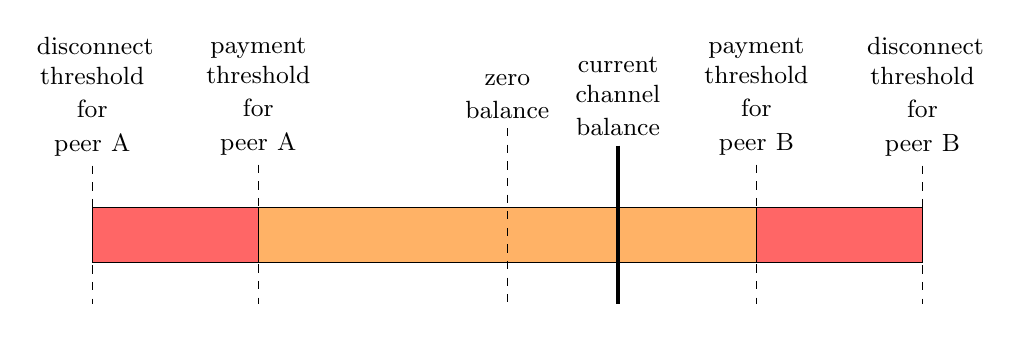
\begin{tikzpicture}
\node (middle)[draw, rectangle, fill=orange!60, minimum height=2em, minimum width=18em]{};
\node (leftred) [draw, rectangle, fill=red!60, minimum height=2em, minimum width=6em, node distance=12em,left of=middle]{};
\node (rightred)[draw, rectangle, fill=red!60, minimum height=2em, minimum width=6em, node distance=12em,right of=middle]{};
\node (zero) [above of=middle,node distance=5em, text width=4em, align=center] {\small zero\\ balance};
\node (zerod) [below of=middle] {};
\draw [dashed](zero)--(zerod);
\node (rtol) [node distance=9em,right of=zero,text width=4em, align=center] {\small payment\\threshold\\for peer B};
\node (rtold) [node distance=9em,right of=zerod] {};
\node (ltol) [node distance=9em,left of=zero,text width=4em, align=center] {\small payment\\threshold\\for peer A};
\node (ltold) [node distance=9em,left of=zerod] {};
\node (rdis) [node distance=15em, right of=zero,text width=4em, align=center] {\small disconnect\\threshold\\for peer B};
\node (rdisd) [node distance=15em,right of=zerod] {};
\node (ldis) [node distance=15em, left of=zero,text width=4em, align=center] {\small disconnect\\threshold\\for peer A};
\node (ldisd) [node distance=15em,left of=zerod] {};
\node (rbal) [node distance=4em,right of=zero,text width=4em, align=center] {\small current\\channel\\balance};
\node (rbald) [node distance=4em,right of=zerod] {};

\draw [dashed](rtol)--(rtold);
\draw [dashed](ltol)--(ltold);
\draw [dashed](rdis)--(rdisd);
\draw [dashed](ldis)--(ldisd);
\draw [very thick](rbal)--(rbald);
\end{tikzpicture}
\end{center}
\caption{Swap balance and swap thresholds.
Zero balance in the middle indicates consumption and provision are equal.
The current channel balance represents the difference in uncompensated service provision:
if to the right of zero, the balance tilts in favour of A with peer B being in debt, whereas to the left
the balance tilts in favour of B with A being in debt.
The orange interval represents loss tolerance. If the balance goes over the payment threshold, the party in
debt sends a cheque to its peer, if it reaches the disconnect threshold, the peer in debt is disconnected.}
\label{fig:swap}
\end{figure}
\end{center}


Extended with a delayed payment instrument like the chequebook, swap also offers a way to deal with unequal consumption
as well as high variance.
In the presence of high variance, or unequal consumption of services, the balance will eventually tilt significantly toward one peer. In this situation, the indebted
party issues a cheque to the creditor, to return the nominal balance to zero. This process is automatic and justifies swap as \emph{settle (the balance) with automated payments}
(see figure \ref{fig:swap}).

Such cheques can be cashed immediately by being sent to the issuer's chequebook contract. Alternatively, cheques can also be withheld
%. Withholding a cheque is effectively lending on credit, 
which enables the parties to save on transaction costs.
While, strictly speaking, there are no solvency guarantees, a bounced cheque will affect the issuer's reputation (as the chequebook contract records it).
On the premise that cheques are swapped in the context of repeating dealings, peers will refrain from
issuing cheques beyond their balance. In other words, interest in keeping good reputation with their peers is an incentive for maintaining solvency.

\begin{center}
\begin{figure}
\begin{center}
\begin{tabular}{ccc}
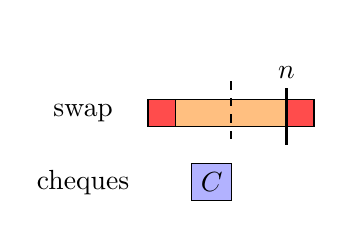
\begin{tikzpicture}
\node (middle)[draw, rectangle, fill=orange!50, minimum height=1em, minimum width=4em]{};
\node (leftred) [draw, rectangle, fill=red!70, minimum height=1em, minimum width=1em, node distance=2.5em, left of=middle]{};
\node (rightred)[draw, rectangle, fill=red!70, minimum height=1em, minimum width=1em, node distance=2.5em, right of=middle]{};
\node (zero) [above of=middle,node distance=2em, text height=1em] {};
\node (zerod) [below of=zero, node distance=3.5em] {};
\node (balance) [right of=zero,node distance=2em, text height=1.5em] {$n$};
\node (balanced) [below of=balance,node distance=3.5em] {};
\draw [dashed](zero)--(zerod);
\draw [very thick](balance)--(balanced);
\node (payment) [below of=zerod, node distance=1em]{};
\node (cheqeue) [draw, left of=payment, node distance=.7em, minimum height=1em, minimum width=1.4em, fill=blue!30, rectangle]{$C$};

\node (swap) [left of=leftred,minimum width=1em,align=right]{swap};
\node (cheques) [below of=swap,minimum width=1em, node distance= 2.5em, align=right]{cheques};
\end{tikzpicture}
&
\begin{tabular}{c}
  $\Longrightarrow$
\\ \\ \\ \\
\end{tabular}
&
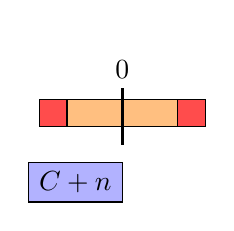
\begin{tikzpicture}
\node (middle)[draw, rectangle, fill=orange!50, minimum height=1em, minimum width=4em]{};
\node (leftred) [draw, rectangle, fill=red!70, minimum height=1em, minimum width=1em, node distance=2.5em, left of=middle]{};
\node (rightred)[draw, rectangle, fill=red!70, minimum height=1em, minimum width=1em, node distance=2.5em, right of=middle]{};
\node (zero) [above of=middle,node distance=2em, text height=1.5em] {$0$};
\node (zerod) [below of=zero, node distance=3.5em] {};
% \draw [dashed](zero)--(zerod);
\draw [very thick](zero)--(zerod);
\node (payment) [below of=zerod, node distance=1em]{};
\node (cheque) [draw, left of=payment, node distance=1.7em, minimum height=1em, minimum width=3.4em, fill=blue!30, rectangle]{$C+n$};
\end{tikzpicture}
\end{tabular}
\end{center}

\caption{Peer B's swap balance (with respect to A) reaches the payment threshold $n$ (left),
B sends a cheque to peer A. B keeps the cheque and restores the swap balance to zero.}
\label{fig:chequeswap}
\end{figure}
\end{center}

\subsection{Cancelling Cheques}

If the imbalance in the swap channel is the result of high variance as opposed to unequal consumption, after a period of accumulating cheques the channel balance starts tilting the other way. Normally it is now up to the other party to issue cheques to its peer resulting in uncashed cheques accumulating on both sides.
To allow for further savings in transaction costs, it could be desirable to be able to `play the cheques off against each other'.

Such a process is possible, but it requires certain deep changes within the chequebook contract. In particular, cashing cheques can no longer be immediate and must incur a security delay, familiar to anyone who has studied other implementations of payment channels.

Let us imagine a system analogous to cheques being returned to the issuer.  
Assume peer A issued cheques to B and the balance was brought back to zero. Later the balance tilts in A's favour but the cheques from A to B have not been cashed. In the real world, user B could simply return the last cheque back to A. In our case it is not so simple; we need some other mechanism by which B commits not to cash that particular cheque. Such a commitment could take many forms; it could be implemented by B signing a message allowing A to issue a new `last cheque` which has a lower cumulative total amount than before, or perhaps B can issue some kind of `negative` cheque for A's chequebook.

What all the implementations have in common, is that the chequebook can no longer allow instantaneous cashing of cheques. Upon receiving a cheque cashing request, the contract must wait to allow the other party in question to submit potentially missing information about cancelled cheques or reduced totals. 

We describe one possible implementation below.

\subsubsection{Waiving debt: bidirectional payments using a single chequebook }\label{subsubsec:waivingdebt}

To accommodate (semi-)bidirectional payments using a single chequebook we make the following modifications

\begin{enumerate}
    \item All cheques from user A to user B must contain a serial number.
    \item Each new cheque issued by A to B must increase the serial number.
    \item A's chequebook contract records the serial number of the last cheque that B cashed.
    \item During the cashing delay, valid cheques with higher serial number supersede any previously submitted cheques regardless of their face value.
    \item Any submitted cheque which decreases the payout of the previously submitted cheque is only valid if it is signed by the beneficiary.
\end{enumerate}

With these rules in place it is easy to see how cheque cancellation would work. 


Suppose user A has issued cheques $c_0 \ldots c_n$ with cumulative totals $t_0 \ldots t_n$ to user B. Suppose that the last cheque B cashed was $c_i$. The chequebook contract has recorded that B has received a payout of $t_i$ and that the last cheque cashed had serial number $i$.

Let us further suppose that the balance starts tilting in A's favour by some amount $x$. If B had already cashed cheque $c_n$, then B would now have to issue a cheque of her own using B's chequebook as the source and naming A as the beneficiary. However, since cheques $c_{i+1} \ldots c_n$  are uncashed, B can instead send to A a cheque with A's chequebook as the source, B as the beneficiary, with serial number $n+1$ and cumulative total $t_{n+1} = t_n - x$. Due to the rules enumerated above, A will accept this as equivalent to a payment of amount $x$ by B.

This process can be repeated multiple times until the cumulative total is brought back to $t_i$. At this point all outstanding debt has effectively been cancelled and any further payments must be made in the form of a proper cheque from B's chequebook to A.


\textbf{Suggestion - delete the rest of this subsection.}


In this scenario, instead of sending a cheque to A, B can waive part of their entitlement. This justifies swap as \emph{send waiver as payment} (see figure \ref{fig:waiverswap}).
A waiver essentially implements a proof that a cheque is destroyed and cannot be cashed, i.e., a promise that (part of) an uncashed cheque will not be redeemed.

A \gloss{waiver} is implemented as a note signed by the peer holding uncashed cheques %. The note specifies the current \gloss{swap index} (sequential number) 
 and indicates the amount of debt they agree to waive from their entitlement.

% \subsubsection*{Cashing cheques in the context of waivers}
If a channel is set to issue waived cheques then cashing must be a two step process.
Upon receiving a cheque, the contract verifies the data, and %signature and checks if the swap index matches the one on the cheque.
if the cheque is valid, the claimed amount is stored in a variable along with a timestamp. At this point a grace period starts: the original issuer gets notified of the cashing request and is invited to send in their last (highest) waiver signed by their peer. In case waivers are allowed cheques specify a \gloss{swap cycle index} and the contract keeps track of this.

% \subsubsection*{Cashing waivers}
Analogously to cheques, waivers are accepted by the contract. %if sent in as data in a transaction together with the issuer's address.
Upon receiving a waiver the contract verifies the data, and checks if the swap cycle index matches the one in the waiver.
If the waiver is valid, the peer's cumulative cashed balance is increased by the waived amount pretending the waived amount was paid out. Then the new cumulative cashed balance is compared to the one recorded when the cheque was received. Any remaining positive balance is transferred to the beneficiary, the cumulative sum is cleared from storage and the swap cycle index is incremented.

%%I stop here for now because the use of 'the swap index'  is confusing and I will rewrite it later ot be more clear.... a sequential index of waivers, stored by the checkbook separately from the serial number of the cheques but functioning like... how should this work? unclearly written

During the grace period the amount is not checked against the book's global balance.
After the grace period expires and no waiver was received, a second transaction
increments the swap cycle index and simply releases the funds or defaults on its debt.
During the grace period, further cheques can be sent to the contract: if they are valid and have the same swap cycle index as the one currently recorded, they simply replace the earlier one and the grace period is renewed.
Since waivers need to match the swap cycle index set by the cheques they destroy, they cannot be sent to the contract before the cheques they waive or after a new swap cycle starts.

In normal operation, however, peers are not incentivised to send in cheques as long as they can issue waivers. Once the waiver goes over the total amount of uncashed cheques, the peer needs to send a cheque. The swap cycle index is incremented in this cheque and the basis for issuing is the channel balance stored on the chain. This makes sure that cheques and waivers cannot be reused.%
%
\footnote{The volume of cheques waived will not increase the cumulative balance and therefore do not count toward total business volume for the purposes of credit history.
This can be amended if cheques are sent together with the latest waivers
and after validation the contract would adjust the cumulative balance to reflect the total volume.}

Using waivers can substantially increase the tolerated variance in the channel balance
without requiring actual transfer or impacting liquidity of the chequebook.
Without it, both peers would need to issue cheques and settlement would involve
transferring back and forth between the two peers, which means the first amount cashed
would not be available for a party for a period.

Waived cheques represent stronger guarantees since the cheque can effectively serve
as backing for incurring costs dedicated to the original issuer.

To summarise, Swap is ideally suited for immediately verifiable, recurring micropayments for bidirectional
services. The primary use case is bandwidth compensation and accounting to incentivise
relaying in a peer-to-peer system. As two peers are doing continuous business
they swap services, cheques and waivers and keep accounting and compensation offchain.




\begin{center}
\begin{figure}
\begin{center}
\begin{tabular}{ccc}
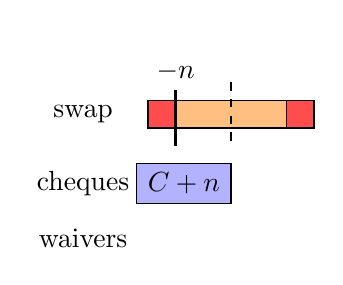
\begin{tikzpicture}
\node (middle)[draw, rectangle, fill=orange!50, minimum height=1em, minimum width=4em]{};
\node (leftred) [draw, rectangle, fill=red!70, minimum height=1em, minimum width=1em, node distance=2.5em, left of=middle]{};
\node (rightred)[draw, rectangle, fill=red!70, minimum height=1em, minimum width=1em, node distance=2.5em, right of=middle]{};
\node (zero) [above of=middle,node distance=2em, text height=1em] {};
\node (zerod) [below of=zero, node distance=3.5em] {};
\node (balance) [left of=zero,node distance=2em, text height=1.5em] {$-n$};
\node (balanced) [below of=balance,node distance=3.5em] {};
\draw [dashed](zero)--(zerod);
\draw [very thick](balance)--(balanced);
\node (payment) [below of=zerod, node distance=1em]{};
\node (cheque) [draw, left of=payment, node distance=1.7em, minimum height=1em, minimum width=3.4em, fill=blue!30, rectangle]{$C+n$};

\node (swap) [left of=leftred,minimum width=1em,align=right]{swap};
\node (cheques) [below of=swap,minimum width=1em, node distance= 2.5em, align=right]{cheques};
\node (waivers) [below of=cheques,minimum width=1em, node distance= 2em, align=right]{waivers};
\end{tikzpicture}
&
\begin{tabular}{c}
  $\Longrightarrow$
\\ \\ \\ \\
\end{tabular}
&
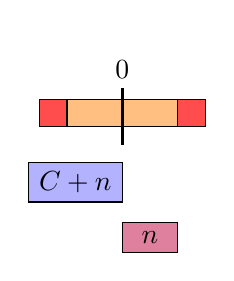
\begin{tikzpicture}
\node (middle)[draw, rectangle, fill=orange!50, minimum height=1em, minimum width=4em]{};
\node (leftred) [draw, rectangle, fill=red!70, minimum height=1em, minimum width=1em, node distance=2.5em, left of=middle]{};
\node (rightred)[draw, rectangle, fill=red!70, minimum height=1em, minimum width=1em, node distance=2.5em, right of=middle]{};
\node (zero) [above of=middle,node distance=2em, text height=1.5em] {$0$};
\node (zerod) [below of=zero, node distance=3.5em] {};
% \draw [dashed](zero)--(zerod);
\draw [very thick](zero)--(zerod);
\node (payment) [below of=zerod, node distance=1em]{};
\node (cheque) [draw, left of=payment, node distance=1.7em, minimum height=1em, minimum width=3.4em, fill=blue!30, rectangle]{$C+n$};
\node (waivers) [below of=payment, node distance=2em]{};
\node (waiver) [right of=waivers,minimum width=2em, node distance=1em,rectangle,draw,fill=purple!50]{$n$};
\end{tikzpicture}
\end{tabular}
\end{center}

\caption{Peer A's swap balance (with respect to B) reaches the payment threshold $n$ (left),
A sends a waiver to peer B. B keeps the waiver and restores the swap balance to zero}
\label{fig:waiverswap}
\end{figure}
\end{center}




\subsection{Using the chequebook one half of a payment channel}
The prototypical payment channel consists of a smart contract set up by two parties A and B. The contract has some number of ether locked up in it that A and B have deposited and the contract keeps track of which portion of the locked up ether belongs to each party. The two parties A and B can exchange signed messages that would (if submitted to the channel contract) change the balance of ownership. Many such messages can be sent back and forth and function as payments between the two parties. Crucially, most of these messages do not need to be submitted to the contract at all. Parties may submit a new state to the channel at any time in order to `save the current state on-chain', but only when one party wishes to actually withdraw ether from the channel does the last message indicating the current `state' of the channel - i.e. the balance between A and B - \emph{have} to be submitted.

A chequebook contract implementing a debt waiving procedure like the one outlined in section \ref{subsubsec:waivingdebt} shares a lot of the same features. If user A has deployed such a chequebook and is using it to pay user B, then the cheques act very similarly to the payment messages above. Key differences to a full payment channel are

\begin{enumerate}
    \item Initially payments can only flow in one direction (from A to B) and the balance can never go `below zero` i.e. in A's favour. This is analogous to a payment channel in which the initial deposit was made only by A.
    \item Balances cannot be updated on-chain without a transfer.
    \item Payout is not guaranteed. 
\end{enumerate}

The fact that payout is not guaranteed is a result of the fact that cheques can bounce (see section \ref{subsec:simple-chequebook}). However it is possible to add a payout guarantee to the cheques on a per-user basis.

\subsubsection{Per-user guarantees}

The chequebook deployed by user A has a balance of ether that acts as collateral for all outstanding cheques A has issued. As such, any user B holding a cheque from A has no guarantee that payout will be possible at any particular time in the future. 

To add a payout guarantee, A would need to make only small modifications to the contract. Explicitly, in order to be able to issue guaranteed cheques to user B, the contract would contain some ether that is locked in the contract and acts as collateral for payments from A to B only. Any cheques held by B are thus guaranteed to be honoured up to this locked amount. Indeed, the only way A can withdraw the locked amount would involve a payout request by A followed by a grace period during which B is still able to submit any outstanding cheques.

With this mechanism in place, the chequebook is now almost equivalent to a full payment channel (albeit one in which the entire initial deposit was made by A).

Note: If both A and B have such a chequebook contract, each having some collateral locked up for the other, then this setup is of functionally equivalent to a full payment channel; with the exception that states can not be `save on-chain' without an actual transfer. In a real payment channel the contract can update the relative balance - how much of the tied up collateral belongs to A and how much belongs to B - but in the chequebook implementation such a re-balancing necessarily involves a transfer from one chequebook contract to the other. Furthermore, advanced payment channels such as Raiden \cite{citation-needed:Raiden} have the ability to string together individual channels and compose them into a network.

Nevertheless, the simplicity of the chequebook implementation has some advantages of its own: the ability to gradually add features as they are needed and the ability to onboard new users at zero cost to them.


\textbf{Suggestion: delete the rest of this subsection}


If the variance is expected to be higher than the loss a peer can afford,
risk of insolvency can be mitigated by assigning part of the balance to a beneficiary.
This locked up sum, called \gloss{channel deposit} allows the owner a tilted balance and
serves as assured collateral dedicated to a particular peer.
This can be implemented by keeping peer-specific balances in the chequebook contract.
This deposit is no longer pooled over multiple creditors
and locking it can guarantee successful cashing of cheques up to the deposited amount.
Withdrawal from the channel deposit is possible but involves a grace period during which
the counterparty is invited to challenge the current balance by sending in the (last) cheque
with the highest amount. After the grace period the owner can reduce the deposit to cover only
its actual debt and may withdraw the remainder.
In order to get the balance of account between peers, the contract needs access to the counterparty
chequebook contract. For ease of explanation we assume that beneficiary is the
chequebook contract itself. Channel deposits can then be implemented as a map with beneficiary contract
address as key and the integer balance in wei as value.

Two chequebook contracts that have a record for each other constitute what is
called a \gloss{payment channel}.


\begin{center}
\begin{figure}
\begin{center}
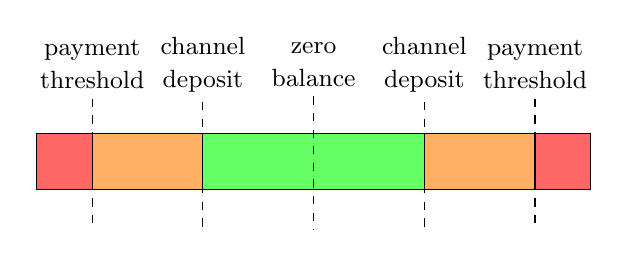
\begin{tikzpicture}
  \node (middle)[draw, rectangle, fill=green!60, minimum height=2em, minimum width=8em]{};
  \node (midleft)[draw, rectangle, fill=orange!60, minimum height=2em, minimum width=4em, node distance=6em, left of=middle]{};
\node (midright)[draw, rectangle, fill=orange!60, minimum height=2em, minimum width=4em, node distance=6em, right of=middle]{};
\node (leftred) [draw, rectangle, fill=red!60, minimum height=2em, minimum width=2em, node distance=9em,left of=middle]{};
\node (rightred)[draw, rectangle, fill=red!60, minimum height=2em, minimum width=2em, node distance=9em,right of=middle]{};
\node (zero) [above of=middle,node distance=3.5em, text width=4em, align=center] {\small zero\\ balance};
\node (zerod) [below of=middle] {};
\draw [dashed](zero)--(zerod);
\node (rtol) [node distance=8em,right of=zero,text width=4em, align=center] {\small payment\\threshold};
\node (rtold) [node distance=8em,right of=zerod] {};
\node (ltol) [node distance=8em,left of=zero,text width=4em, align=center] {\small payment\\threshold};
\node (ltold) [node distance=8em,left of=zerod] {};
\node (prtol) [node distance=4em,right of=zero,text width=4em, align=center] {\small channel\\deposit};
\node (prtold) [node distance=4em,right of=zerod] {};
\node (pltol) [node distance=4em,left of=zero,text width=4em, align=center] {\small channel\\deposit};
\node (pltold) [node distance=4em,left of=zerod] {};
\draw [dashed](rtol)--(rtold);
\draw [dashed](ltol)--(ltold);
\draw [dashed](prtol)--(prtold);
\draw [dashed](pltol)--(pltold);
\end{tikzpicture}
\end{center}
\caption{}
\label{fig:paymentchannel}
\end{figure}
\end{center}

\subsection{Zero barrier to entry}

A tremendous advantage of swap accounting in cinjunction with a chequebook contract %upgraded to function as such a simple payment channel 
is that new users can begin to provide services and earn rewards without owning any ether initially.

Swap accounting can also work in one direction only. If a party enters the system with zero ether (\gloss{newcomer}), but connects to peers with funds and chequebooks (\gloss{insider}), the newcomer begins to provide the service (and not use it)
in order to earn a positive swap balance. Once the payment threshold is reached, the newcomer will be paid and is then able to deploy chequebook of their own\footnote{There is a caveat here in that cashing cheques requires a gas expenditure (although this restriction may fall once ethereum is upgraded to the `Metropolis' release in which the chequebook contract will be able to pay for the transfer and deduct the cost of the transfer from the payout}.

Even without any chequebook contract at all, Swap allows for zero cost onboarding of newcomers. Once the payout threshold is reached, the insiders could pays the newcomers on-chain. 

If a newcomer connects to  an insider with an existing chequebook contract,
the insider agrees to create a chequebook contract for the newcomer
in return for consuming newcomers services. In this scenario, when an insider's service debt reaches the amount needed for contract creation, the insider sends a transaction to create the contract with newcomer as the owner. Once a node has its own chequebook contract, they are able to consume and potentially pay out more to their creditor.

In order to use the contract, however, it makes sense to have a balance on it. Since the owner has no ether, it makes sense to expect that the insider peers with funds will be the ones who deposit this starting balance. If peers agreed that they want to save on transaction costs, it is reasonable to create the contract with the required initial balance in one go. This would imply waiting out with contract creation until the insider's debt reaches the \emph{cost of bootstrapping} which is the sum of (1) the cost of contract creation, (2) the required starting balance, and (3) some extra service fee to incentivise insiders to lend.

With the global deposit included, this cost of bootstrapping
can be substantially higher than nodes' loss tolerance.
If the contract is deployed to the blockchain in advance, with ownership granted
to the newcomer, the newcomer can just move with their new topped-up wallet
to other peers leaving the lender node with loss.
If it is to be deployed only after newcomer provided service totalling
the cost, then the insider node will disappear after essentially leeching on
the newcomer.

Luckily, there is a safe protocol to tackle
bootstrapping: the newcomer issues a cheque to the insider in advance with an amount
corresponding to the bootstrapping cost. Insider creates a contract with herself as owner
and a channel deposit also dedicated to herself in the amount
on the cheque. At this point if the two peers never meet, the newcomer suffered no loss,
the insider can just offer the contract to the next newcomer. Otherwise the service goes
exactly the way as if the newcomer was an insider with a contract, and the insider held
non-cashed cheques, i.e., as the insider consumes, each time it reaches the
payment threshold, it issues waivers against the withheld cheques. This is equivalent
to the insider setting up a subscription with newcomer, authorising withdrawal
with the waivers (see figure \ref{fig:bootstrapping}).

\begin{center}
\begin{figure}
\begin{center}
\end{center}
\caption{Bootstrapping or how to launch as a swap capable node consuming and providing a
service  and earn money}
\label{fig:bootstrapping}
\end{figure}
\end{center}


As newcomer provides service and insider issues waivers, it is business as usual.
Newcomer provides service to other peers and accepts payments sent to the
contract. If the inpayments are insufficient to get the balance up
to cover the bootstrapping cost, the entire contract is still owned by the insider
who can reuse it with another peer with previous inpayments counting as profit.
In this case neither the cheque nor the waivers are valid, therefore all the service insider
may have received was free.

If the balance goes above the cost of bootstrapping, the insider can cash it with
the original cheque which will automatically change the owner to newcomer.
The cheque works exactly as normal, i.e., when cashed, it is stored in escrow
while the contract receives waivers.
Waivers can be used to first cover the difference between channel deposit and balance, and above that
count to reduce the outpayment to insider. In normal operation, once waivers goes over
the cost of bootstrapping, insider issues ???

This system is complete if newcomers have a way to send waivers to the contract.
Since newcomers have zero balance, they cannot bear the transaction   cost and need others to send it for them. 
Waivers and cheques can be signed by their beneficiary. These variants are also accepted by the chequebook
and instruct the contract to pay an amount to the transaction sender covering the transaction cost plus a small service fee.  This way the prospect of the bounty serves as an incentive to
third party insiders to transact on behalf of newcomers.
The waiver or cheque triggers outpayment from the chequebook global  balance to the owner.
This is how to earn ether with a service starting from nothing in the most efficient way.
Signed notes are not only useful for newcomers; anyone without a blockchain connection
will be able to interact and provide services without losing the security of the blockchain.

To summarise, by serving before consuming, participants can
bootstrap their way into swap without the need for funds.
Hence swap is justified as (\emph{setting up a wallet as payment}).


\section{Escrow conditions on future payments}

\gloss{Promissory notes} represent redeemable promises of payment potentially maturing in the future. We define the general notion of a note as a promise that entitles a beneficiary to future payment under a condition. Since this effectively puts the money in an escrow, the condition can also be referred to as an \gloss{escrow condition}. A promissory note can contain the following optional fields:

  \begin{itemize}
    \item swap cycle index
    \item amount
    \item beneficiary
    \item escrow address
    \item valid from
    \item valid until
    \item remark
  \end{itemize}

In the simplest case no escrow condition or maturation date is given: such a note represents a simple cheque as discussed above. The maturation date (blockheight or timestamp) can be specified to indicate the earliest
possible occasion a note can be redeemed (valid from) as well as a deadline when the promise expires unless its escrow condition is satisfied (valid until). 

\subsection{Recurring payments}

The cheque represents an adhoc promise to redeem an amount. The transfer of funds is sanctioned by a cheque issued for each occasion. There is, however, services where recurring payments are predictable and therefore the installments can be sanctioned in advance. The primary usecase is subscription services. This could be implemented by storing a whitelist of contract addresses that are allowed to withdraw from the chequebook balance. For simplicity, however, we choose to represent this analogously to cashing a cheque. Authorising a recurring payment to a contract is done by signing a blank cheque (a cheque with an unspecified amount) against the beneficiary possibly with a valid until date. Such beneficiaries are smart contracts and therefore no defense against false amount is needed. Receiving transfer request transactions is independent of the swap state of cumulative amount and simply withdraws the amount from the global balance or the channel deposit of the owner.

\subsection{Bonds}

A note with an amount and beneficiary and a future valid from data is effectively a bond. The amount factors in all outstanding payment obligations the beneficiary is entitled to once the bond matures including interest. When such a note is not collateralised at the time of issuing, accepting the bond is equivalent to granting a loan on the grounds of the credit history of the account. 
\subsection{Escrow conditions and escrow witnesses}

If an escrow address is specified in the note, the referenced contract can be used to verify the condition of redemption. When the escrow condition is verified, the owner, the beneficiary address, and the note id (the hash of the signed note) are passed as arguments to the {\gloss{testimonyFor}} method of the escrow contract. By implementing this method the contract conforms to the \gloss{witness} contract  interface (section \ref{sec:courtroom}). Given the witness contract, the escrow condition is implicitly defined as whatever state makes the escrow witness give a positive testimony. 

A note with an escrow field specified is called a \gloss{conditional bond} and can represent a \gloss{service contract} with the escrow condition describing successful delivery. In a real-life scenario, upon verification of an instance of service provision or purchase of a good, the escrow acknowledges the delivery before releasing the funds. This is implemented by the chequebook calling the escrow witness contract to give a testimony. In case the condition is fully verifiable algorithmically in the VM, the entire transaction remains within the closed system, there is no real-world liability and the transfer is enforceable.

If no beneficiary is specified, a conditional note is essentially a \gloss{bounty}. A bounty is meant to be published or broadcast to a set of known service providers. Bounties will play a crucial role in certain types of service networks, discussed in section \ref{sec:wasp}. Figure \ref{fig:taxonomy} summarises the various types of promissory notes.


\newcommand{\tick}{\checkmark}
\newcommand{\opt}{?}
\begin{center}
\begin{figure}
\begin{center}
\begin{tabular}{|l|r||c|c|c|c|c|c|c|}
\hline
note & fields
& swap cycle index
& amount
& beneficiary
& escrow
& valid from
& valid until
& remark
\\
\cline{2-9}

type & type 
& int256
& int256
& address
& address
& int256
& int256
& byte32
\\
\hline
\hline
\multicolumn{2}{|l||}{cheque}   & \tick & \tick & \tick & & & \opt& \opt
\\
\multicolumn{2}{|l||}{authorisation} &  & \tick & \tick & & & \opt& \opt
\\
\multicolumn{2}{|l||}{bond} & \tick & \tick & \tick & & \tick & \opt& \opt
\\
\multicolumn{2}{|l||}{conditional bond} &  & \tick & \tick & \tick & \tick & \opt& \opt
\\
\multicolumn{2}{|l||}{bounty} & \tick &  \tick & & \tick & \tick & \opt& \opt
\\
\multicolumn{2}{|l||}{soft channel deposit} &  \tick & \tick & & & && \opt
\\
\hline
\end{tabular}
\end{center}
\caption{Taxonomy of promissory notes: '\tick' indicates a mandatory field, types show the corresponding solidity type to encode in the ABI. '?' indicates optional field.}
\label{fig:taxonomy}
\end{figure}
\end{center}


% \subsection{Secure escrow and liquidity}

\subsection{Conditional bond, invoice, and cheque}

Let us assume that node A issues a conditional note (or bounty) to B with expiry at time T.
T represents the earliest time that A can consider the note unfulfilled (the service undelivered), before
that we say that the note is \emph{active}.

If B fulfills the condition, it notifies A of successful delivery
by sending an \gloss{invoice} containing the hash of the note and the current cumulative balance they want the
amount to be added to. The invoice is supposed to represent the balance at delivery, and serves to
indicate that the subsequent cheque will be the one to pay the outstanding amount for the note.
As a response A is expected to send a cheque with an updated channel balance reflecting the
payment of the invoice (the amount in the conditional note is added to the cumulative total).
If A refuses to do this, B can send the conditional note in a transaction
to  the contract. When the witness validates the delivery condition, and the testimony is
positive, the amount goes to escrow and a grace period starts.
During the grace period, A can settle the claim by sending in the appropriate cheque.

If the note condition does not check out, B's challenge will cost them the transaction.
Even if it does, they won't gain anything by the challenge if they did receive the
cheque from A since they still needed to send the proof in a transaction.
Therefore B is disincentived to initiate frivolous challenges.
Conversely, A is incentivised to send the cheque to B after it receives the invoice,
otherwise it is A that needs to pay the transaction cost of sending in the cheque upon B's correct challenge.
We therefore conclude that the optimal behaviour for A and B is offchain exchange of invoice and cheque.

\subsection{Soft channel deposits}
A nonmaturing cheque is a deposit locked up as collateral to secure varying balance.
The total value of these deposits serve as guaranteed collateral for any debt and
therefore conceptually equivalent to a channel deposit.
In the following we describe a construct which gives 100$\%$ guarantee of solvency
on outstanding conditional bonds without explicitly assigning deposits to channels on chain.%
%
\footnote{In the on-chain case channel deposits are explicitly stored in the contract, therefore overspending
(using the amount to collateralise multiple creditors) is impossible.}

Let us assume A and B both maintain an ordered list of active conditional notes issued by A.
Each time A issues a conditional note or pays for a fulfilled one or one expires, the list is updated.
The hashes of active notes in order of issuance is organised in a swarm tree, the
root hash of which is signed by B and passed to A together with a so called
\gloss{soft channel deposit claim}. This claim constitutes an acknowledment of
the outstanding liabilities of A towards B. Assume further that there exist a notion of \gloss{epoch},
a fixed settlement period at the end of which B needs to sign off on the total sum of active
outstanding conditional notes issued by A to B.
Formally, soft channel deposit claim is a note with the following fields:

\begin{itemize}
  \item A's contract address
  \item the total sum of all active outstanding conditional notes
  \item the epoch index
\end{itemize}

With each epoch, B signs the note and sends it to A.
Peer A can verify if the soft claim is correct and terminate dealings if not. In such a case soft claim of
the last epoch is taken, whereby A cancels its liability to the conditional notes issued since
the last epoch.
B is incentivised to send the correct soft claim if they want business with A fulfilling their
conditional notes.

After A receives soft channel deposit claims from all peers for the epoch, the claims are
collected in a list (ordered according to the peer index of the beneficiary in A's swap contract).
A signs the swarm hash of the (concatenated) list and sends it alongside the list
in a construct called a \gloss{soft channel deposit allocation table} to each peer.
Upon receiving the soft channel deposit allocation table, B verifies that
(1) the total sum of channel deposits allocated is no greater than the global deposit and
(2) the amount dedicated to B is no less than the sum of all outstanding active
conditional notes issued by A to B.
(3) each active peer in A's swap contract has a corresponding claim for the current epoch and the signature is valid.
This process in illustrated in figure \ref{fig:softchanneldeposit}


\begin{center}
\begin{figure}
\begin{center}
\begin{tikzpicture}
\end{tikzpicture}
\end{center}
\caption{Soft channel deposit}
\label{fig:softchanneldeposit}
\end{figure}
\end{center}




At any point in time, soft channel deposit claims can be consolidated to actual
channel deposits.
The soft channel deposit claim is sent in with the inclusion proof of the claim against the root hash of the
current channel deposit allocation table as a transaction to the
chequebook contract. Upon receiving and validating the claim (signature, resource and epoch verified),
the contract simply reallocates the claimed amount from the global deposit to the channel.
If each peer does this, the global deposit is reduced with the total of soft channel
deposits.%
%
\footnote{To save all peers the trouble of sending inclusion proofs, when A initiates withdrawal from
their global deposit, they need to submit current allocation table starting a grace period during which
creditors are invited to challenge the allocation by presenting a contradicting claim.}

Once the channel deposit (of A towards B) is secured on chain, all the outstanding conditional notes
issued to B are guaranteed to be redeemable in the standard ways.
If a peer is found to issue contradictory channel claims for the same epoch, they relinquish
their right to any claim. For any third party this entails that if a peer's claim is
included in the allocation table, the maximum they are entitled to redeem is limited to:
(1) the sum in the claim if they signed a correct unique claim or
(2) zero if they illegally signed multiple claims for the same epoch.
Futhermore, the allocation table is exhaustive, therefore each
peer signed their claim and no peer without a channel deposit are allowed to have a claim. 
From this, third parties can also conclude that the sum of all claims in the
allocation table is the maximum total deposit that can be consolidated as channel deposits.
In order to secure full liability, it is stipulated in the validity criteria of allocation tables, that the sum of allocations do not exceed the global soft channel deposit.

If the soft channel deposit allocation table is valid,
we can with complete certainty know that the global deposit in A's contract
 could cover all outstanding conditional notes handed to B even if all peers were to redeem all of their outstanding notes (e.g., by satisfying A's conditional bond).
Practically this means then that, after receiving a valid allocation table for the epoch from A,
B has no risk of insolvency when dealing with A's conditional notes.
To insure a completely risk-free flow of conditional notes, the peers only  need to make sure that the total of their outstanding nodes do not exceed the sum of the current soft channel  deposit and the on-chain channel  deposit. 
In fact nodes reallocate soft channel deposits to channels where they suspect that in the following epochs the total outstanding amount from conditional bonds and bounties will increase beyond what the channel deposit can cover and deallocate away from the channel if they are not expected to.
Therefore in a way, hard channel deposits play the role of the payment  threshold in simple swap, whereas soft channel deposits serve are somewhat analogous to cheques or waivers for service-specific collateral against issued service requests. 

In sum, using soft channel deposits enables the chequebook owner to allocate and reallocate funds
as channel deposits in a fairly flexible way without blockchain transaction costs,
yet provide $100\%$ solvency guarantees on all active conditional bonds and bounties to their peers.


\section{Service guarantees}
\label{sec:courtroom}

In the previous section we introduced tools to compensate service providers.
While rewards are paid out only if delivery is successful, such positive incentivisation may be insufficient if explicit guarantees of future delivery are required.

In this section we describe a system of service contracts and dispute resolution.
Service contracts allow providers (or a set of providers) to offer quality and/or delivery guarantees to customers. First we describe how to give service guarantees (swear), then discuss how they can be enforced (swindle). Finally we link together the three contracts by showing how the swap interacts with swear and swindle.


\subsection{Commitment and litigation}

Without loss of generality, we can conceptualise a generic service as described by a game contract on the blockchain (see later in \ref{sec:swindle}).


Nodes indicate their \gloss{commitment} to providing a service by signing against the game contract either in a transaction or issuing a signed note offchain. By committing to the game contract  providers can be challenged if they don't comply with the rules.

Litigation on the other hand, allows customers to initiate an on-chain court procedure in case they suspect foul play. Such accountability is crucial for the design of scalable decentralised service economies.

We will describe the trial process for dispute resolution and how it evaluates the evidence against the accused provider. The verification is the same as the one used in the context of sanctioning outpayments when the escrow condition is evaluated after service delivery. However, if a provider is proven guilty by the court on the grounds of not complying with the rules specified in the service contract, various punitive measures will be automatically enforced. In most cases, this comprises losing some deposit that provider previously locked up as collateral to back their promise.%
%
\footnote{Instead of or in addition to losing their deposits, nodes would also suffer loss of reputation. If any demonstrated violation of terms is recorded on the public blockchain, users can expect clean histories as a measure of reputation.}
%
By registering on a service contract and putting up a deposit if required, providers \emph{swear} to play by the rules. This deposit is locked up and used later as compensatory insurance transferred to the customer, redistributed or burnt.

\subsection{Trial}
\label{sec:swindle}

If a service provider is suspected of non-compliance, they can be challenged by opening a case with the swear contract analogous to filing a case and have it 
tried in the courtroom.
An abstract trial is composed of stages of litigation, at each stage the court procedure calls witnesses and, depending on their testimony, advances the trial into the next stage. Witnesses can refuse testimony if evidence is not (yet) available in which case the trial is paused until the grace period allowed to submit evidence is over. Eventually the trial concludes with a guilty or not guilty verdict followed by automatically enforced punitive measures in the former case or compensation to the accused in the latter.

The specific service contract describes the rules of the service by assigning particular expert witnesses to trial stages. These witnesses evaluate evidence submitted to them in relation to the case and give testimony if asked by the judge.
The request--response process between the judge and the witnesses can thus be standardized even though each witness may require different data to be submitted to them as evidence.

To implement such an abstract dispute resolution system, the trial is described by a \emph{finite state automaton} the states of which correspond to stages of litigation. The transitions are labelled with various outcomes of evaluating evidence submitted to the respective expert witness associated with the stage (true, false, N/A). A witness is a smart contract that implements the \emph{testimony} function which takes as arguments the provider address, the plaintiff address, and the note id (the hash of the signed note) representing the service request.

The \gloss{swindle} contract orchestrates the transition through the stages by calling the witness contracts, handles grace periods to control the deadline for submitting evidence (challenges or their refutations) to eventually reach a guilty/non-guilty verdict on the grounds of witness testimonies.
In case of a guilty verdict, the deposit sworn on is forfeited and the peer's registration is terminated as executed by the swear contract.

\begin{center}
\begin{figure}
\begin{center}
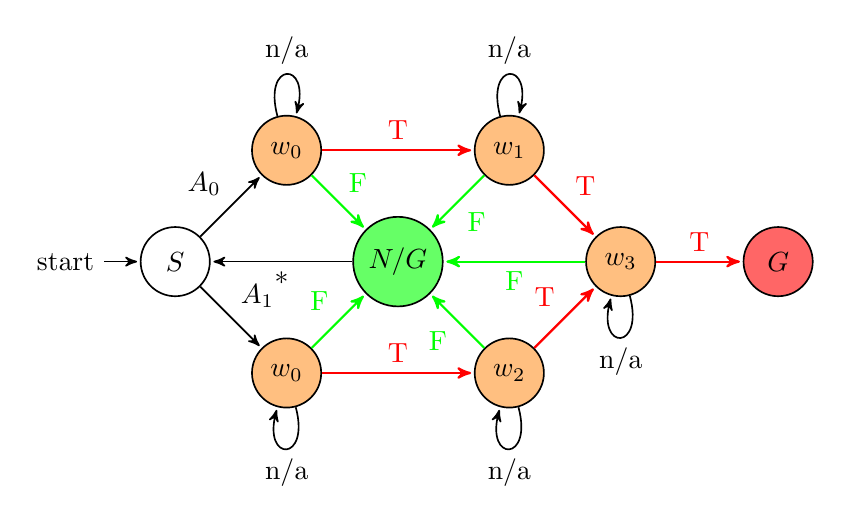
\begin{tikzpicture}[->,>=stealth',shorten >=1pt,auto,node distance=2c m,
                    semithick]
  \tikzstyle{witness}=[fill=orange!50,draw]
  % \tikzstyle{every state}=[fill=gray!10,draw]

  \node[initial,state] (S)                    {$S$};
  \node[state,witness]         (W0_1) [above right of=S] {$w_0$};
  \node[state,witness]         (W0_2) [below right of=S] {$w_0$};
  \node[state,fill=green!60]         (N/G) [below right of=W0_1] {$N/G$};
  \node[state,witness]         (W1) [above right of=N/G] {$w_1$};
  \node[state,witness]         (W2) [below right of=N/G] {$w_2$};
  \node[state,witness]         (W3) [below right of=W1] {$w_3$};
  \node[state,fill=red!60]         (G) [right of=W3]       {$G$};

  \path (S) edge   node {$A_0$} (W0_1)
            edge   node {$A_1$} (W0_2)
        (W0_1) edge [loop above] node {n/a} (W0_1)
            edge [red,thick]             node {T} (W1)
            edge [green,thick]             node {F} (N/G)
        (W0_2) edge [loop below] node {n/a} (W0_2)
            edge [red,thick]             node {T} (W2)
            edge [green,thick]             node {F} (N/G)
        (W1) edge [loop above] node {n/a} (W1)
            edge [red,thick]             node {T} (W3)
            edge [green,thick]             node {F} (N/G)
        (W2) edge [loop below] node {n/a} (W2)
            edge  [red,thick]            node {T} (W3)
            edge  [green,thick]            node {F} (N/G)
        (N/G) edge              node {*} (S)
        (W3) edge [loop below] node {n/a} (W3)
            edge  [green,thick]            node {F} (N/G)
            edge [red,thick]  node {T} (G);
\end{tikzpicture}
\end{center}
\caption{Trial stages represented as a finite state automaton describing a service contract. Upon receiving an accusation ($A_0$ or $A_1$) in a transaction, the case contract moves to the first litigation state. The orange circles represent states where a witness contract is called, the following state depends on the outcome of the witness testimony (the return value of the $\mathit{testimony}$ function call).
The other nodes call the internal $\mathit{process}$ function: to pay compensation if the challenge is refuted (N/G) or enforce the sentence in case of a guilty verdict (G).}
\label{fig:servicecontract}
\end{figure}
\end{center}

\subsection{Enforcement}

When a guilty verdict is reached, the swindle contract calls back to the swear contract to enforce the sentence, the forfeiture of the game deposit. The swear contract acts as executor of this decree, in a way similar to how a court order is observed by the agencies in a position to enforce sentences.  

The contract that handles the deposits and registers which node plays which game is called \gloss{swear}.
The swear contract is a registry of commitments, a mapping from identities to game contracts.%
%
\footnote{One can imagine not completely open swear registries which curate a whitelist of safe or recommended games. Similarly to an appstore, these contracts could catalogue service games.}
%
An entry is created if a provider signs off on a service game contract in an act of \gloss{commitment}. Essentially, the swear contract only needs to record how much deposit each commitment promised and let the swap channel handle the deposit.
The swear contract can  ask the swap if the provider has insufficient funds dedicated as swear deposits. This is simply implemented by channel deposit allocation: nodes allocate the appropriate amount as channel deposit with the swear contract as beneficiary.%
%
\footnote{If the grace period for withdrawal from hard channel deposits is implemented by a call to the channel beneficiary, then we can handle in an elegant way the cases where deposits are locked as collateral for services with arbitrary validity period.}
%
Commitments are implemented as a signed note containing an amount, the swear contract address as the escrow witness, the games contract address in the remark field, optionally a beneficiary and validity dates. Commitments are a subtype of conditional bonds which when submitted to the swap, call out to the swear contract as its witness and starts a new case against the issuer. 
Interpreted as a service request, a commitment authorises the transfer of a balance up to the amount (actual amount determined by the witness) and asks the swear contract to handle all service complaints against the provider. The swear contract implements the witness interface and when its \emph{testimony} function is called, it prepares the case and authorises the swindle contract to lead the trial. When the guilty or not-guilty verdict is reached, the swindle contract calls back to the swear contract that sets out to execute the sentence with a call to $execute$ giving a case id as argument.

The sentence starts with transferring the deposit amount to the deposit handler contract calling \emph{execute} with the case id.


In this section we connected the dots and showed how swap swear and swindle interact.
The swap contract can validate promissory notes so it can itself serve as witness for the swindle contract.
When a commitment is sent to the swap contract, it calls the swear contract as an escrow witness which in turn opens a case and sanction the swindle contract to lead a trial.
Once the verdict is reached, the sentence is executed by the swear contract which has authorisation to withdraw the deposit from the swap contract that holds it in the form of hard channel deposit. Figure \ref{fig:sw3} gives an  overview of these interactions.

\begin{center}
\begin{figure}
\begin{center}
\begin{tikzpicture}
\end{tikzpicture}
\end{center}
\caption{Swap, Swear and Swindle contracts and their interactions:
}
\label{fig:sw3}
\end{figure}
\end{center}

\section{Service networks}
\label{sec:networks}

In this section we describe how the tools for peer-to-peer accounting and data exchange can be used to drive the incentives for distributed digital services. Assume that a set of nodes form a network that provides a decentralised service. Insured chunk storage in swarm, arbitrary remote payments or database insertion are examples of such services. 
A \gloss{service task} is defined as an instance of service provision. Storing a particular chunk, paying an amount to another node or inserting an entry to an index are examples of tasks of the respective network service.

In what follows we will work with the assumption that the participating nodes in a service network are connected in a \gloss{kademlia topology} and can relay messages to other nodes using kademlia deterministic routing based on direct devp2p transport layer for each hop. In other words service networks are composed of a subset of nodes within swarm.

Scalability of swap channels is based on the premise that directly connected nodes engage in long-term repeated dealings and can afford setting up contracts on the blockchain to secure their interaction.%
%
\footnote{Given the semi-permanent connections of the TCP based kademlia of swarm, peers interact with $O(log(n))$ peers where $n$ is the number of nodes in the network.}
%
A \gloss{swap channel network} enables \gloss{indirect transactions} by relaying tasks and deliveries using swap-channel transactions on every hop. This makes it possible to preserve the scalability and security of swap, yet extend the scope of transactions both in terms of frequency and reach, i.e., enabling \emph{ad-hoc one-off interactions} between \emph{any two non-connected nodes}. 
Service networks with global provision guarantees (introduced in section \ref{sec:wasp}) further improve the scope by offering guaranteed market making and delivery in a direct immediately settling swap transaction. As a result, service users can just \emph{request and disappear}.

\subsection{Incentivisation for relaying}

[This section may not be part of this article, but the one on relaying etc]

Let's assume that nodes A,B,C,D are participant peers of a service network such that
A-B, B-C and C-D are direct connections with a swap channel.
Assume further that A intends to do some ad-hoc one-off business with D. To this end,  A issues a conditional bond specifying an escrow condition that some data be obtained from D constituting the proof of delivery of the task.

When A sends the conditional bond to B as beneficiary, B receives the conditional bond and issues the same bond only this time with C as beneficiary. C is directly connected to D, so it just relays the same to D who issues a receipt (or takeover proof). 
Each of these steps is implemented as swaps of conditional notes. The moment C receives the receipt, it is incentivised to pass it back to B as an invoice to prompt settlement. The same is true for B and any number of intermediate relaying nodes (see figure \ref{fig:svcnets-sequence-diagram}).

% \PreviewEnvironment{tikzpicture}
% \setlength\PreviewBorder{7pt}
\definecolor{pinegreen}{cmyk}{0.92,0,0.59,0.25}
\definecolor{royalblue}{cmyk}{1,0.50,0,0}
\definecolor{violet}{cmyk}{0.79,0.88,0,0}
\tikzstyle{cblue}=[circle, draw, thin,fill=cyan!20, scale=0.8]
\tikzstyle{qgre}=[rectangle, draw, thin,fill=green!20, scale=0.8]
\tikzstyle{rpath}=[thin, densely dotted, black, opacity=0.7]
\tikzstyle{gpath}=[thick, pinegreen, opacity=0.4]
\tikzstyle{dpath}=[ultra thin, black, opacity=0.4]
\tikzstyle{legend_isps}=[rectangle, rounded corners, thin, 
                       fill=gray!20, text=blue, draw]
                        
\tikzstyle{legend_overlay}=[rectangle, rounded corners, thin,
                           minimum width=2.5cm, minimum height=0.8cm,
                           pinegreen]
\tikzstyle{legend_phytop}=[rectangle, rounded corners, thin,
                          minimum width=2.5cm, minimum height=0.8cm,
                          royalblue]
\tikzstyle{legend_general}=[rectangle, rounded corners, thin,
                          minimum width=2.5cm, minimum height=0.8cm,
                          violet]
\tikzstyle{node_label}=[rectangle, thin,
                          minimum width=0.2cm, minimum height=0.2cm,
                          black]
\tikzstyle{node_legend}=[rectangle, thin,
                          minimum width=1.2cm, minimum height=0.2cm,
                          black]

% Diagram
\begin{figure}
\centering
   

\begin{tikzpicture}[auto, thick]
 % Cloud creation
  \node[cloud, fill=gray!20, cloud puffs=16, cloud puff arc= 100,
        minimum width=7cm, minimum height=2.5cm, aspect=1] at (0,0) {};

 % Physical layer nodes
  \foreach \place/\x in {{(-2.5,0.3)/1}, {(-1.75,-0.55)/2},{(-1.2,0.55)/3},
    {(-0.75,-0.7)/4}, {(-0.25,0)/5}, {(0.25,0.7)/6}, {(0.75,-0.3)/7}, 
    {(1.5,0)/8},{(2.5,0.4)/9}}
  \node[cblue] (a\x) at \place {};
 
 % Physical layer links
  \path[thin] (a1) edge (a2);
  \path[thin] (a1) edge (a3);
  \path[thin] (a2) edge (a3);
  \path[thin] (a3) edge (a6);
  \path[thin] (a2) edge (a4);
  \path[thin] (a5) edge (a6);
  \path[thin] (a5) edge (a4);
  \path[thin] (a5) edge (a2);
  \path[thin] (a5) edge (a7);
  \path[thin] (a6) edge (a7);
  \path[thin] (a6) edge (a9);
  \path[thin] (a6) edge (a8);
  \path[thin] (a8) edge (a9);
  \path[thin] (a7) edge (a8);
 


\node[node_label] (A) at (-2.5,2.6) {A};
\node[node_label] (B) at (-1.2,2.85) {B};
\node[node_label] (C) at (0.75,1.6) {C};
\node[node_label] (D) at (2.25,2.3) {D};

%swap connection legend nodes
\node (LS) at (4.2,1.4) {};
\node (LE) at (5.2,1.4) {};
\path[gpath] (LS) edge (LE);

 % Overlay layer nodes
  \foreach \place/\i in {{(-2.5,2.3)/1},{(-1.2,2.55)/2},
    {(0.75,1.3)/3}, {(2.25,2)/4}}
    \node[qgre] (b\i) at \place {};
 
 % Overlay layer links
  \path[dpath] (b1) edge (b2);
 % \path[dpath] (b1) edge (b4);
 % \path[dpath] (b2) edge (b4);
  \path[dpath] (b4) edge (b3);
 % \path[dpath] (b3) edge (b1);

  \path[gpath] (b1) edge (b2);
  \path[gpath] (b2) edge (b3);
  \path[gpath] (b3) edge (b4);

 % Links between overlay and physical topology
  %\foreach \i in {1,...,4}
  %  \path[rpath] (a\i) edge (b\i);
  \path[rpath] (a1) edge (b1);
  \path[rpath] (a3) edge (b2);
  \path[rpath] (a7) edge (b3);
  \path[rpath] (a9) edge (b4);
 % Legends
  \node[legend_general] at (0,4){\textsc{Swarm Service Networks}};
  \node[legend_overlay] at (6,2){\textsc{Kademlia Overlay}};
  \node[legend_phytop] at (6,0){\textsc{Physical Network}};
  \node[node_legend, font=\fontsize{4}{4.5}\selectfont] at (6.2,1.4) {Direct Swap Connection};

 
 
\end{tikzpicture}
\caption{Swap channel network: peer to peer network of nodes with semipermanent TCP connections organised in
a kademlia topology. Given nodes have an associated identity owning a chequebook contract,
each live connection defines a swap channel.}
\label{fig:svcnets-overlay-diagram}
\end{figure}

% Agents
\def\A{A}
\def\B{B}
\def\C{C}
\def\D{D}

% Message Flows
\def\BondB{Conditional Bond A->B}
\def\BondC{Conditional Bond B->C}
\def\BondD{Conditional Bond C->D}
\def\ReceiptD{Receipt D->C}
\def\ReceiptC{Receipt C->B}
\def\ReceiptB{Receipt B->A}

% Legend 
%\def\LegendOnChain{On-chain}
%\def\LegendOffChain{Off-chain}

% Diagram
\begin{figure}
\centering
   

% Diagram
\begin{tikzpicture}[every node/.style={font=\normalsize,
  minimum height=.7cm,minimum width=1.5cm},]

% Matrix
\node [matrix, very thin,column sep=.7cm,row sep=0.1cm] (matrix) at (0,0) {
  & \node(0,0) (\A) {};   &                         & \node(0,0) (\B) {};   &                         & \node(0,0) (\C) {};     &                         & \node(0,0) (\D) {}; \\
  & & & & & & & \\
  & & & & & & & \\
  & & & & & & & \\
  & \node(0,0) (\A 1) {}; & \node(0,0) (\BondB) {}; & \node(0,0) (\B 1) {}; &                         & \node(0,0) (\C 1) {};   &                         & \node(0,0) (\D 1) {}; \\
  & & & & & & & \\
  & & & & & & & \\
  & \node(0,0) (\A 2) {}; &                         & \node(0,0) (\B 2) {}; & \node(0,0) (\BondC) {}; & \node(0,0) (\C 2) {};   &                         & \node(0,0) (\D 2) {}; \\ 
  & & & & & & & \\
  & & & & & & & \\
  & \node(0,0) (\A 3) {}; &                         & \node(0,0) (\B 3) {}; &                         & \node(0,0) (\C 3) {};   &  \node(0,0) (\BondD) {};& \node(0,0) (\D 3) {}; \\
  & & & & & & & \\
  & & & & & & & \\
  & \node(0,0) (\A 4) {}; &                         & \node(0,0) (\B 4) {}; &                         & \node(0,0) (\C 4) {};   &  \node(0,0) (\ReceiptD) {}; & \node(0,0) (\D 4) {}; \\
  & & & & & & & \\
  & & & & & & & \\
  & \node(0,0) (\A 5) {}; &                         & \node(0,0) (\B 5) {}; & \node(0,0) (\ReceiptC) {};& \node(0,0) (\C 5) {}; &                          & \node(0,0) (\D 5) {}; \\
  & & & & & & & \\
  & & & & & & & \\
  & \node(0,0) (\A 6) {}; & \node(0,0) (\ReceiptB) {};& \node(0,0) (\B 6) {}; &                         & \node(0,0) (\C 6) {};&                          & \node(0,0) (\D 6) {}; \\
  & & & & & & & \\
  & & & & & & & \\
  & \node(0,0) (\A 7) {}; &                         & \node(0,0) (\B 7) {};  &                          & \node(0,0) (\C 7) {};&                          & \node(0,0) (\D 7) {}; \\
  & & & & & & & \\
  & & & & & & & \\
%  & \node(0,0) (\A 7) {}; & \node(0,0) (\LegendOnChain) {};  & & & & & \\
%  & \node(0,0) (\A 8) {}; & \node(0,0) (\LegendOffChain) {}; & & & & & \\
};

% Agents labels
\fill 
	(\A) node[draw,fill=white] {\A}
	(\B) node[draw,fill=white] {\B}
	(\C) node[draw,fill=white] {\C}
	(\D) node[draw,fill=white] {\D};

\draw [dashed] 
  (\A) -- (\A 7)
  (\B) -- (\B 7)
  (\C) -- (\C 7)
  (\D) -- (\D 7);

% Horizontal flows (Monetary interactions)
\draw [-{Latex[length=1mm,width=1.5mm]}] (\A 1) -- (\B 1);
\draw [-{Latex[length=1mm,width=1.5mm]}] (\B 2) -- (\C 2);
\draw [-{Latex[length=1mm,width=1.5mm]}] (\C 3) -- (\D 3);
\draw [-{Latex[length=1mm,width=1.5mm]}] (\D 4) -- (\C 4);
\draw [-{Latex[length=1mm,width=1.5mm]}] (\C 5) -- (\B 5);
\draw [-{Latex[length=1mm,width=1.5mm]}] (\B 6) -- (\A 6);

% Flows Labels 
\fill
  (\BondB) 
    node[above] {\BondB}
  (\BondC) 
    node[above] {\BondC}
  (\BondD) 
    node[above] {\BondD}
  (\ReceiptD) 
    node[above] {\ReceiptD}
  (\ReceiptC) 
    node[above] {\ReceiptC}
  (\ReceiptB) 
    node[above] {\ReceiptB};

% Interaction points 
\draw 
  (\A 1) node[minimum size=0.1cm, draw,circle,fill=red!20] {}
  (\B 1) node[minimum size=0.1cm, draw,circle,fill=red!20] {}
  (\B 2) node[minimum size=0.1cm, draw,circle,fill=red!20] {}
  (\C 2) node[minimum size=0.1cm, draw,circle,fill=red!20] {}
  (\C 3) node[minimum size=0.1cm, draw,circle,fill=red!20] {}
  (\D 3) node[minimum size=0.1cm, draw,circle,fill=red!20] {}
  (\D 4) node[minimum size=0.1cm, draw,circle,fill=red!20] {}
  (\C 4) node[minimum size=0.1cm, draw,circle,fill=red!20] {}
  (\C 5) node[minimum size=0.1cm, draw,circle,fill=red!20] {}
  (\B 5) node[minimum size=0.1cm, draw,circle,fill=red!20] {}
  (\B 6) node[minimum size=0.1cm, draw,circle,fill=red!20] {}
  (\A 6) node[minimum size=0.1cm, draw,circle,fill=red!20] {};

\end{tikzpicture}
\caption{Sequence of conditional bond exchange and receipt forwarding in a service network}
\label{fig:svcnets-sequence-diagram}
\end{figure}

In general, we define an \emph{indirect transaction} as a chain of swaps between directly connected
peers. The success of a such indirect transactions between two nodes is dependent on whether and
how such a chain can be found. Our assumption is that the nodes have semi-permanent connectivity
and form a network topology where routing between any two nodes is guaranteed, e.g., kademlia. As a result, we can assume that as long as all nodes on the chain have a healthy kademlia connectivity, the prerequisite for finding a route is satisfied.

In order to incentivise relaying nodes to take part in such a network, a transaction fee for every hop needs to be introduced.  We stipulate that the transaction fee for one swap is proportional to the logarithmic distance that the hop spans. As a consequence, the simple rational strategy to maximise profit will incentivise nodes to find the closest node when relaying as well as maintain a healthy connectivity needed for successful routing. Furthermore, the entire transaction fee can be precalculated as proportional to the distance between sender and remote beneficiary and therefore can be offered in advance when issuing the conditional bond.

This construct is equivalent to message relaying with \gloss{certified delivery}, except that nodes are required to have funds to cover the amount of the conditional bond.
For live connections in a service network to be operational, parties agree to always having in-channel capacity in the amount of X. With soft channel deposits, such throughput restrictions can easily be relaxed and adjusted even on an on-demand basis.

In addition to swap channels, connected nodes operate \gloss{provable data exchange}. Assume that two nodes participate in a particular service that involves relaying objects (such as requests and responses). The content addresses (swarm hash) of consecutive objects sent in one direction constitute a \emph{data stream}. Both peers save this stream to swarm and maintain an index mapping the hashes to offsets. The upstream peer (sender) calculates the swarm hash of this index and periodically signs it against the current blockheight or timestamp as well as the data stream identitfier. This \gloss{handover state} is periodically sent to the downstream peer (receiver)
who verifies it and preserves it until the next one. The downstream peer periodically countersigns the handover state together with an initial offset or timestamp. This \gloss{takeover state} is then sent to the upstream peer. For instance, the handover state obtained from the upstream peer can be used to prove to third parties that an object X was handed over to the downstream peer. This can be done by giving an inclusion proof of the hash of X.%
%
\footnote{Upstream peer can be challenged to give an inclusion proof.}

On top of the rewards peers get for relaying, we can introduce additional incentives to guarantee that messages reach the recipient. We can assume that relaying nodes register on a service contract they promise to relay messages in a data stream towards the recipient. If nodes have a stake to lose, punitive measures can be imposed on nodes that fail or refuse to relay messages in the data stream.

Take our earlier example of A sending a message to remote node D, and assume that B, C, and D are all registered relaying nodes that are online. If there is reason to believe that the message did not reach D, A can challenge B by simply providing the takeover proof for the message. B can defend itself by providing takeover proof from C, thereby shifting the blame to C for blocking the delivery. C in turn can show takeover proof from D to refute the challenge. It can also happen that C indeed did not forward the message because there was no node closer to D among its peers. But this means that D is a nearest neighbour of C, in which case D should have been connected to C.
Therefore D can be challenged to prove that it was connected to C. D can respond to the challenge
by showing handover state obtained from C dated after the message delivery deadline. This in turn is
a challenge to C to show the inclusion proof of the message against the handover state.
This pattern is called \gloss{finger pointing} and constitutes the investigative part
of litigation which results in identifying the node
ultimately responsible for failed delivery by not relaying.
Finger pointing essentially implements \emph{guaranteed delivery}.

\subsection{Uniform resource allocation and market making}
\label{sec:wasp}

In the previous section we just assumed that A knew about D (from an independent source). In case there are other nodes as well that can in theory perform the same task, a bounty is sent to potentially multiple addresses of candidate providers and an implicit market making mechanism is obtained by certified delivery.

Assume the tasks of a service network can be provided by any participating node using the same amount of resources. Given a network of willing providers, a system can be designed called \gloss{global resource allocation by network topology (GRANT)} such that tasks are distributed more or less uniformly across the network.

For instance, this is the case with storage in swarm: each task of storage provision involves storing a fixed-size chunk of data. We index the chunks with their content address (swarm hash) and allocate the storage task to nodes whose address is closest to the chunk address. Since both nodes and chunks are uniformly distributed in the same address space, this strategy implements uniform load balancing. We can generalise this allocation strategy for any task if requirements are uniform across tasks by simply indexing the task requests with their hash.

When a service user issues a bounty to request a service task, the bounty is sent towards the task's address using kademlia routing. The node responsible for servicing the task is dynamically defined as the closest node at any point in time. If hops use provable data streams, the incentives can make sure that the request (task bounty note) reaches the appropriate nodes and thereby are granted the opportunity to deliver the task.

For continuous services such as chunk storage, this means that as nodes leave and join the network, the node responsible for a task can change over time. With data exchange proofs however, we can enforce that nodes synchronise historical task requests and therefore the allocation can be taken for granted. In other words, the network can perform dynamic load-balancing of previously submitted future tasks even though the network is changing.

In order to benefit from the allocated tasks by cashing the bounties on delivery, the distribution
should be incentivised. In particular relaying nodes are not supposed to withhold tasks in hope of cashing the bounty themselves. To guarantee that downstream peers do get forwarded all the tasks and bounties, upstream peers can be challenged when they cash a bounty: if there is a valid handover proof of connection (synchronisation) for the relevant period after the bond was issued, upstream peer can be challenged for not relaying it (but withholding). Conversely, the bounty outpayment can be challenged if the candidate provider is not the closest node to the task, i.e., a downstream peer closer to the task address can show connectivity during the relevant period. Withholding if proven could result in the same punitive measure as failing to deliver.


Service nodes that are capable of staying online can choose to register and put up a deposit as collateral. One consequence of GRANT is that for each task, there is a node (or set of neighbouring nodes) that is responsible for delivering the task and can ultimately be held liable for non-delivery. Using the swindle scheme for litigation, if proven guilty a node's collateral is forfeited. Since individual punitive measures are a very effective incentive, service guarantees can be given independent of the positive incentivisation (the reward for delivery implicit in the bounty).%
%
\footnote{Since the amount of tasks (and therefore capacity requirements) are roughly uniform for each participant node, catastrophic failure of an entire node can cause limited damage. Since the required deposit is meant to collateralise this risk, it is reasonable to set it to a fixed amount across all provider nodes.}

When the original issuer of the task request receives the receipt for its bounty (takeover proof) from its immediate peer, they have all that is needed to start finger pointing after the deadline for the service task passed. In other words, service users have \emph{instant guarantees} that the service will be provided for the task they request, even though it is unknown at the time by which node.

This type of service network is called \gloss{warranted automatic service provision (WASP)} network.
Since one can thus obtain instant enforceable service guarantees in one swap exchange, WASP networks allow users to \gloss{request and disappear}. Applying this scheme to swarm insured storage, given a WASP network of storage nodes, swarm users can \emph{upload and disappear}.

\subsection{Atomic swap}

The typical market making mechanism is the swap of request, offer, agreement. This pattern is described as a conditional note issued by A specifying an escrow that requires a second conditional bond referring to the first one sent back.  
If this is countersigned by A, the testimony is positive, otherwise N/A.
This construction can be abstracted out as a generic connector witness analogous to the logical AND operator. It validates two conditional notes and checks their mutual commitment to binding them atomically. 

% Another usecase is decentralised orderbooks

\section{Pricing in service networks}

\subsection{Reverse auction for competitive bounties}
\subsection{Signalling capacity overload}
\subsection{Service networks for stablecoins}

\cite{btcmicro2014}
\cite{decker2015fast}
\cite{poon2015bitcoin}  %lightnening
\cite{prihodko2016flare} % routing in lightening
\cite{tremback2015universal}  %paymentchannels
\cite{bonneau2014mixcoin} % anonimity
\cite{ethersphere2016sw3}
\cite{ethersphere2016smash}
\cite{maymounkov2002kademlia}
\cite{heep2010r}
\cite{malavolta2017concurrency}
\cite{chiesa2017decentralized}
\cite{heilman2016tumblebit}
\cite{green2016bolt}
\cite{miller2017sprites}
\cite{mcdonald2017payment}
\cite{diferrante2017payment}

\bibliography{./refs.bib}
\appendix
\section{Swap contract}
\section{Swear and swindle contract}
\section{Swarm storage insurance}
\section{Scaleable node-to-node payments}
\printglossary

\end{document}
